
\section{Service Architecture Models}

Infrastructure as a Service platforms at it's core controls various virtualization interfaces and services and allows to launch a new virtual server from given disk image at chosen host server, connect it to provided physical or virtual network and add block storage device to it. The OpenStack platform provides services that address needed to provide the very basic compute, network and storage services. The identity provider and image store  provide further services needed to provide the basic sevices.

Nebula was the predecessor of OpenStack and was superseded because it did not scale well. The services withing OpenStack communicate through 3 various communication channels

TCP/SQL - Services store it's state in SQL datastore

AMQP - Service internally communicate over asychronous communication bus which .... Compute service calls network service 

HTTP - All services expose REST APIs that allow higher level integration, control ...

\subsection{Architectural Level}

OpenStack is complete Infrastructure as a Service platform. It allows to create virtual servers on virtual networks using virtual block devices.

%Jak funguje IaaS ve smyslu deploye masiny z pohledu controlleru - zavola scheduler, ten comupte, ten pak glance, pak pripadne cinder a neutron a pusti boot, kdyz to ma ready. a tim padem provoz.

\begin{figure}[!h]
\centering
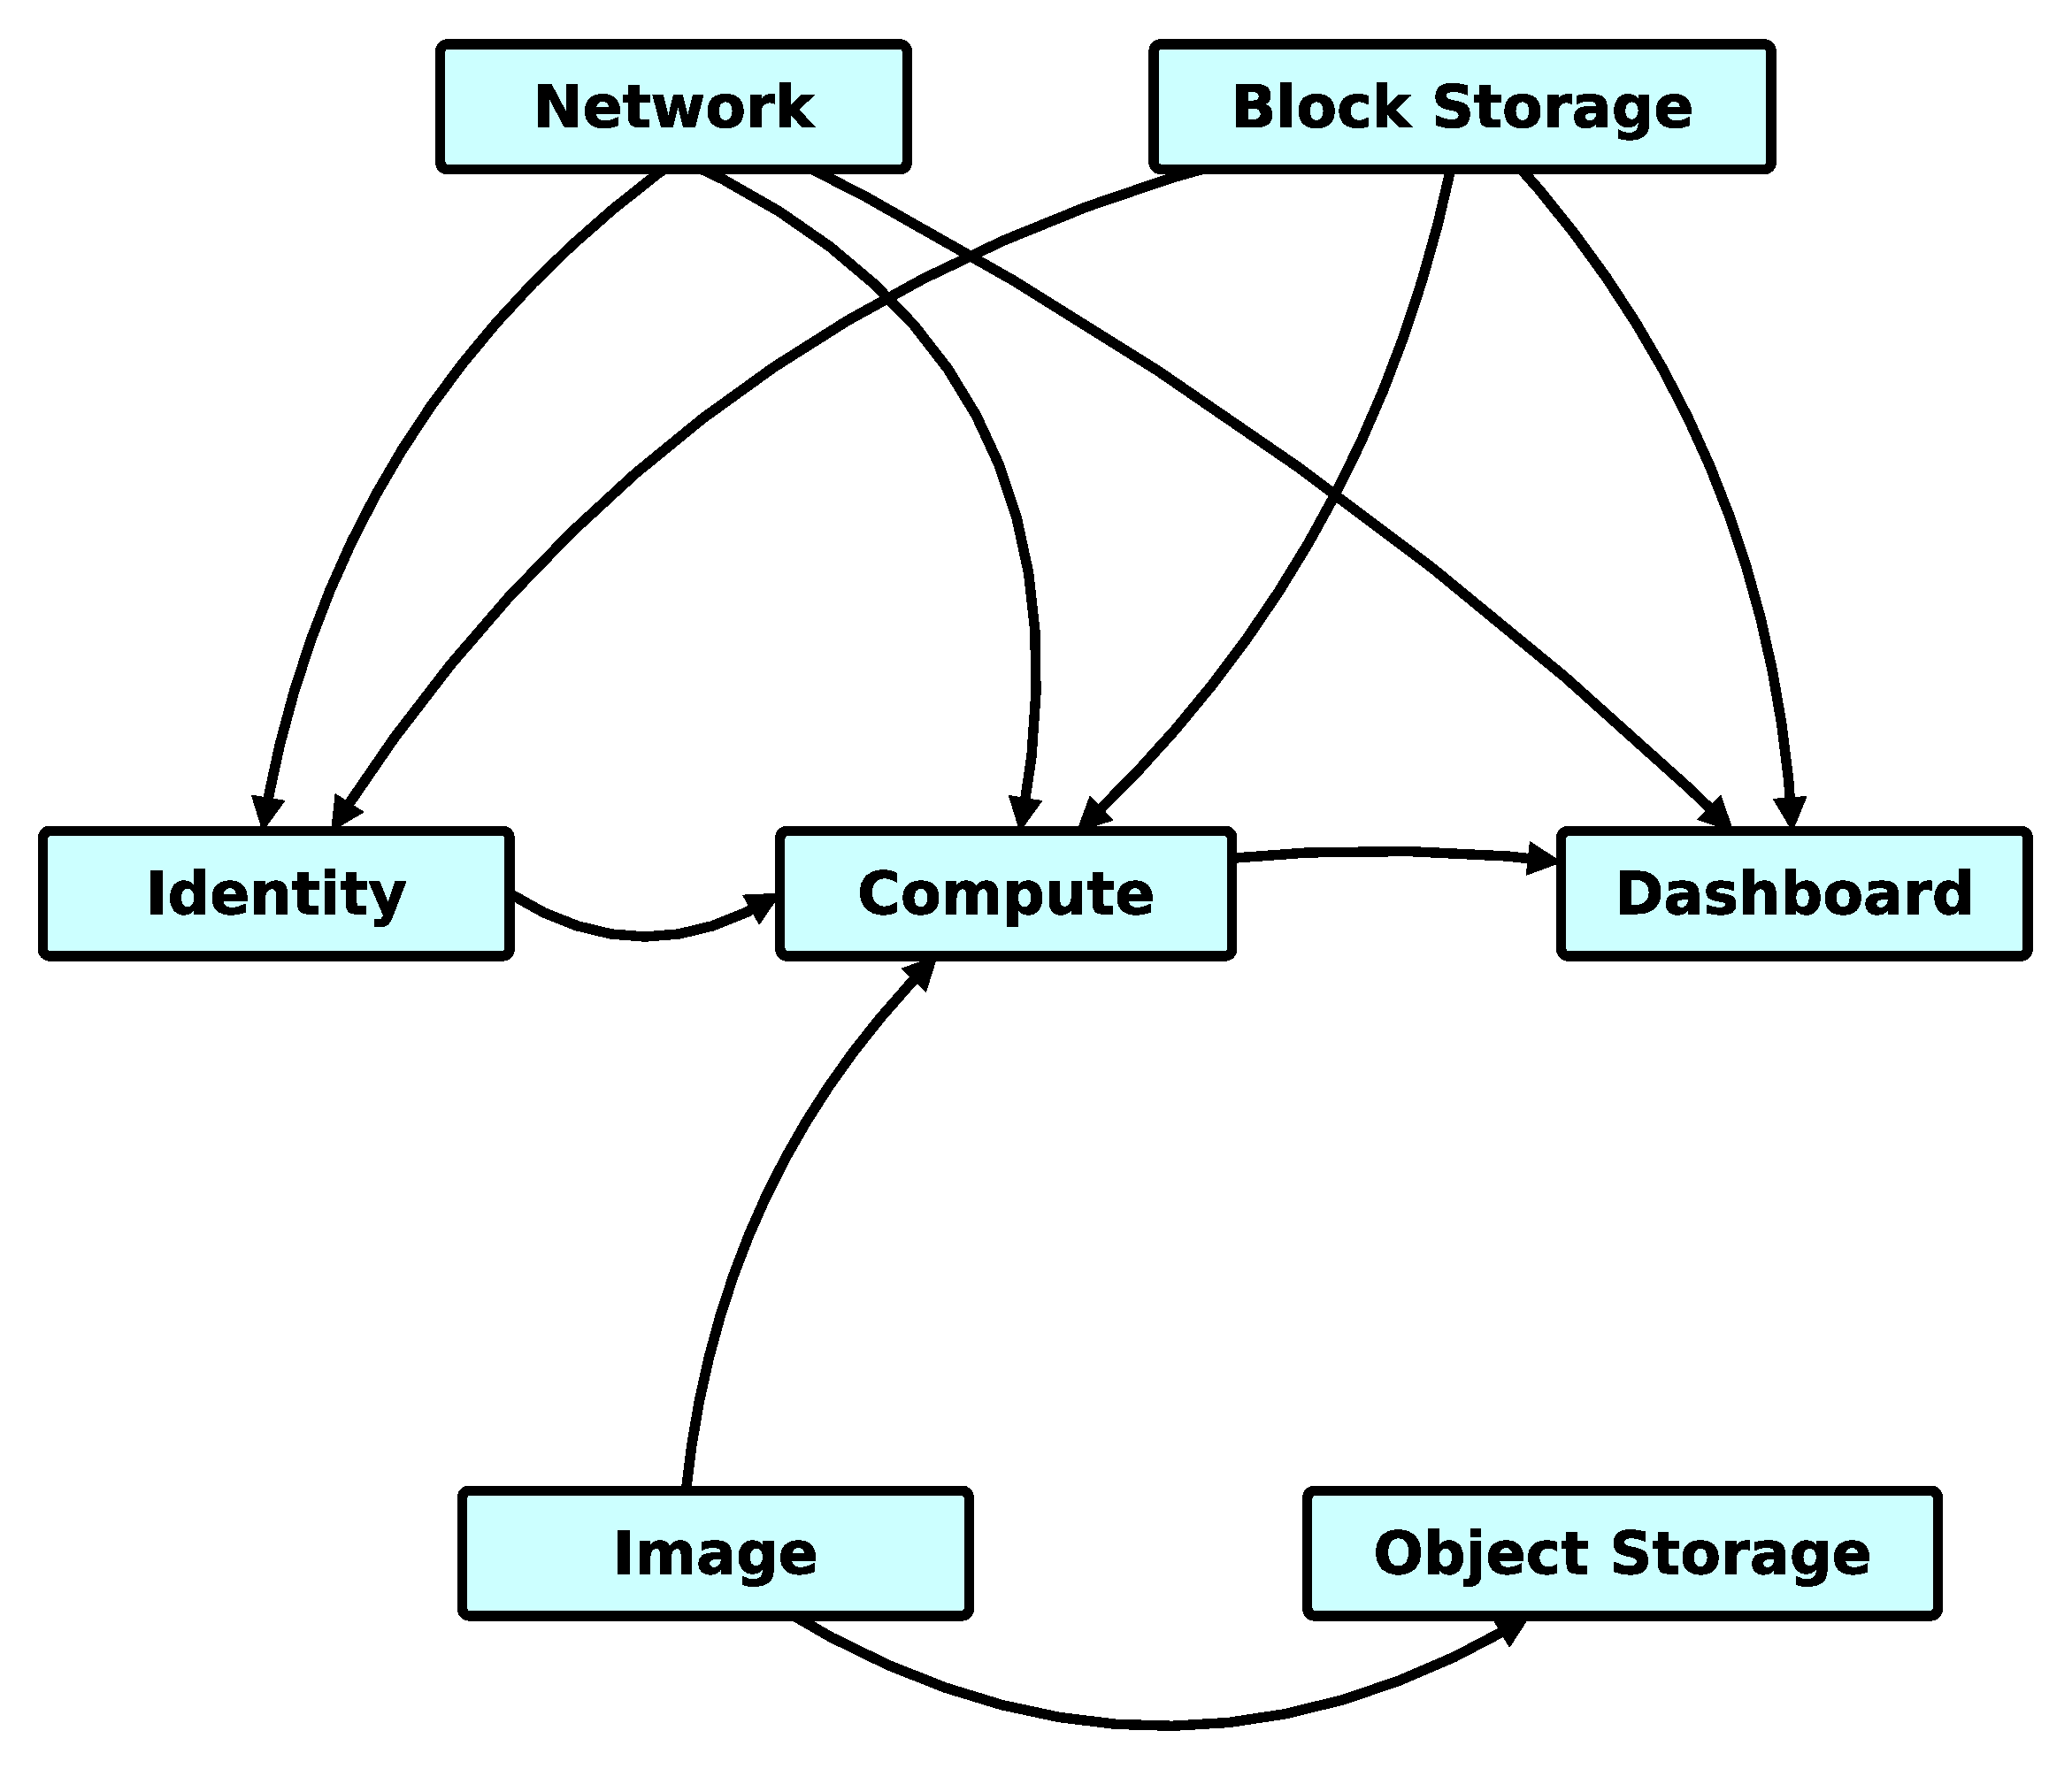
\includegraphics[scale=.2]{img/openstack_logical_model.eps}
\caption{Logical Model of Havana OpenStack}
\label{fig:cm}
\end{figure}

Further versions of OpenStack introduce more sophisticated services that use basic services to Data processsing 

 These core services are followed by growing number of services covering for example telemetry, orchestration or data processing. All services within OpenStack architecture have pluggable backends. This allows vendors to develop plugin for their resources, that can be accessed and managed by the OpenStack API.

Following Figure shows the basic configuration of OpenStack in Icehouse version.

\begin{figure}[!h]
\centering
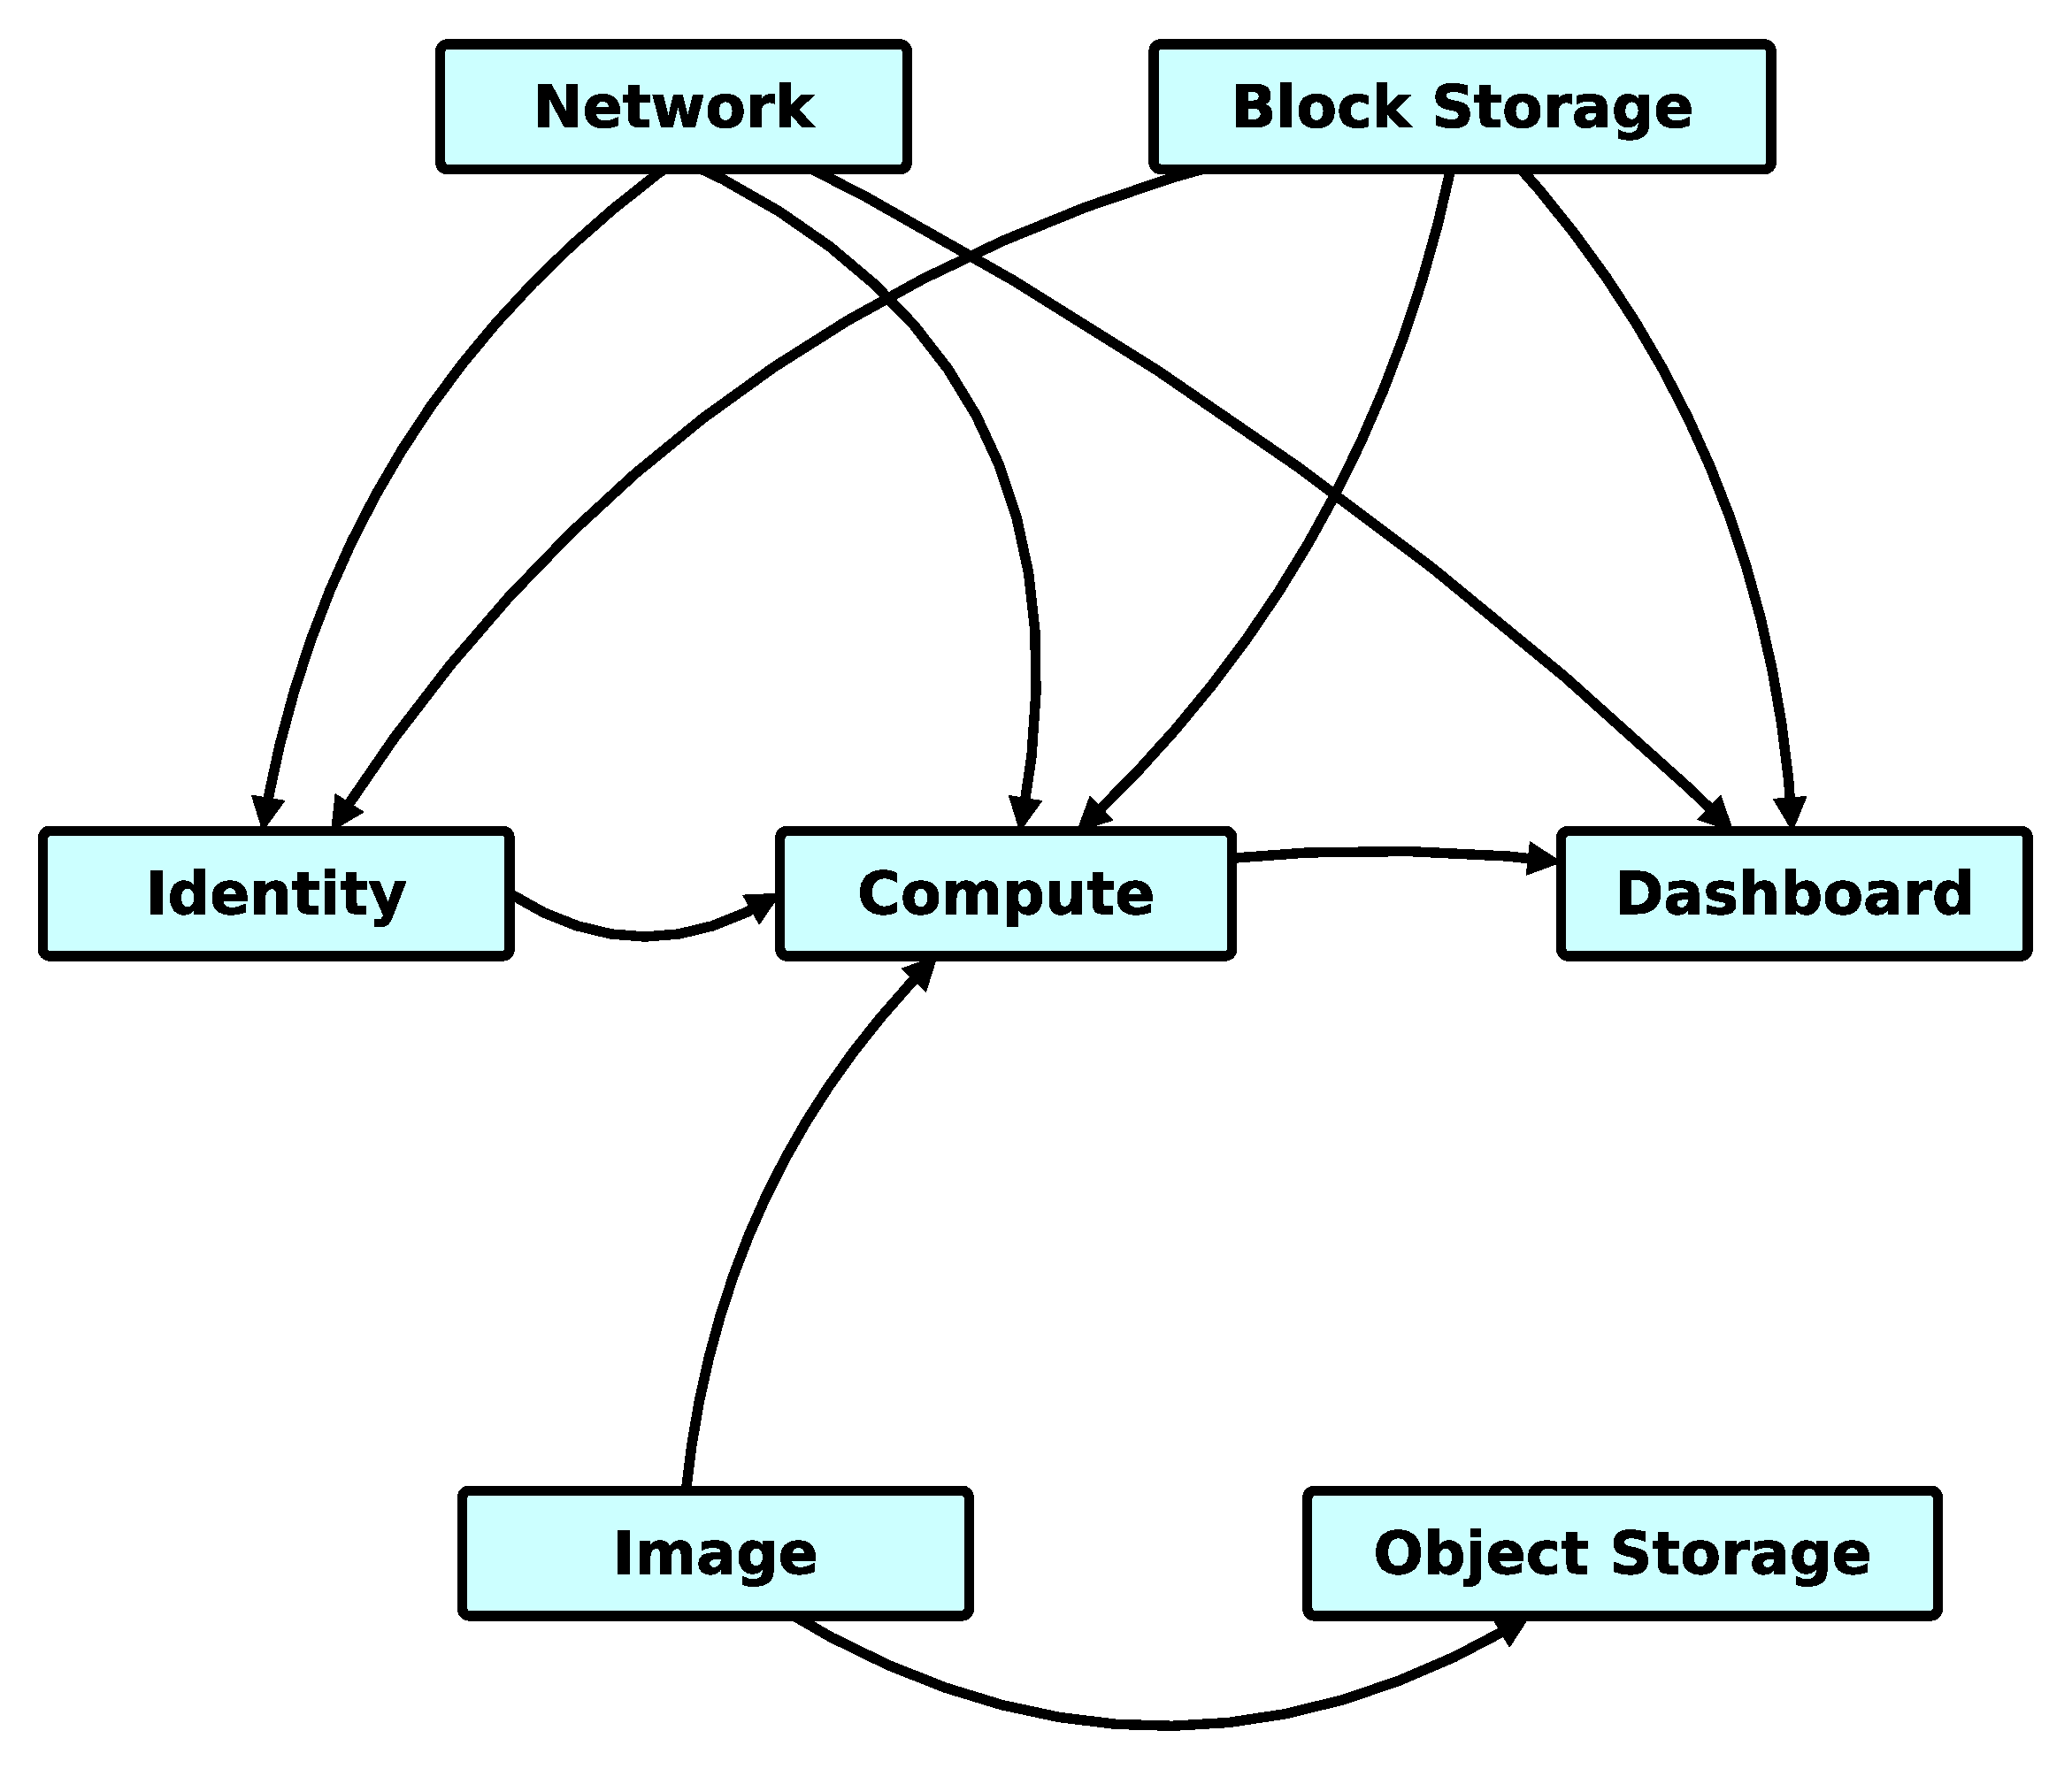
\includegraphics[scale=.2]{img/openstack_logical_model.eps}
\caption{Logical Model of Icehouse OpenStack service achitecture}
\label{fig:cm}
\end{figure}


Klasicky logicky model openstack architektury

2) OpenStack architecture moduls

% Rozebrat services a představit modularitu a vendor plugins, drivers

Database

Message queue

Time service

Identity - Keystone

Image - Glance

Compute - Nova

Network - Neutron

Volume - Cinder

\subsection{IaaS Controller Support Services}

This section covers the 

Real implementations of Architectural models

\subsubsection{High Availability Services}

Cluster software
- corosync/pacemaker
- keepalived

\subsubsection{Communication Services}

RPC

- rabbitmq

- qpid

- 0mq

\subsubsection{Database Services}

Database

- mysql/galera

- postgressql/xtradb

\subsubsection{Time Synchronization Services}

time

- ntp

\subsection{Iaas Controller Core Services}

APIs

Pluggable backends

\subsubsection{Identity Service}

Keystone is an OpenStack project that provides Identity, Token, Catalog and Policy services for use specifically by projects in the OpenStack family.

- sql	

- ldap

\subsubsection{Image Service}

OpenStack Image service (code-named Glance) provides services for virtual disk images. Compute service uses image service to get the starting image of the virtual server.

OpenStack Image service handles variety of disk image formats, including Raw, Machine (kernel/ramdisk outside of image, also known as AMI), VHD (Hyper-V), VDI (VirtualBox), and qcow2 (Qemu/KVM).

- dir

- swift

- s3

\subsubsection{Compute Service}

OpenStack Compute service (code-name Nova) is designed to provision and manage large networks of virtual machines, creating a redundant and scalable cloud-computing platform.  It provides the software required to orchestrate compute instances through using libvirt or or other virtualization client libraries. OpenStack Compute service is both hardware and hypervisor agnostic, currently supporting a variety of standard hardware configurations and major hypervisors.

- kvm

- qemu

- docker

- hyper-v

- vsphere

\subsubsection{Network Service}

Neutron is an OpenStack networking project focused on delivering networking as a service. Neutron has replaced the original networking application program interface (API) in OpenStack. Neutron is designed to address deficiencies in “baked-in” networking technology found in cloud environments, as well as the lack of tenant control (in multi-tenant environments) over the network topology and addressing, which makes it hard to deploy advanced networking services.


- flat networking

- ovs-gre/vxlan

- sdn

  - opencontail
  
  - nsx

\subsubsection{Volume Service}

Cinder

- lvms

- sans

Různé způsoby nasazení ukázky reálné architektury - promapovat ve 4 na ontologii

\subsection{Use Cases}

Why we choose different openstack setups

\subsubsection{Locality 1}

At CEPSOS laboratory have deployed 

\begin{figure}[!h]
\centering
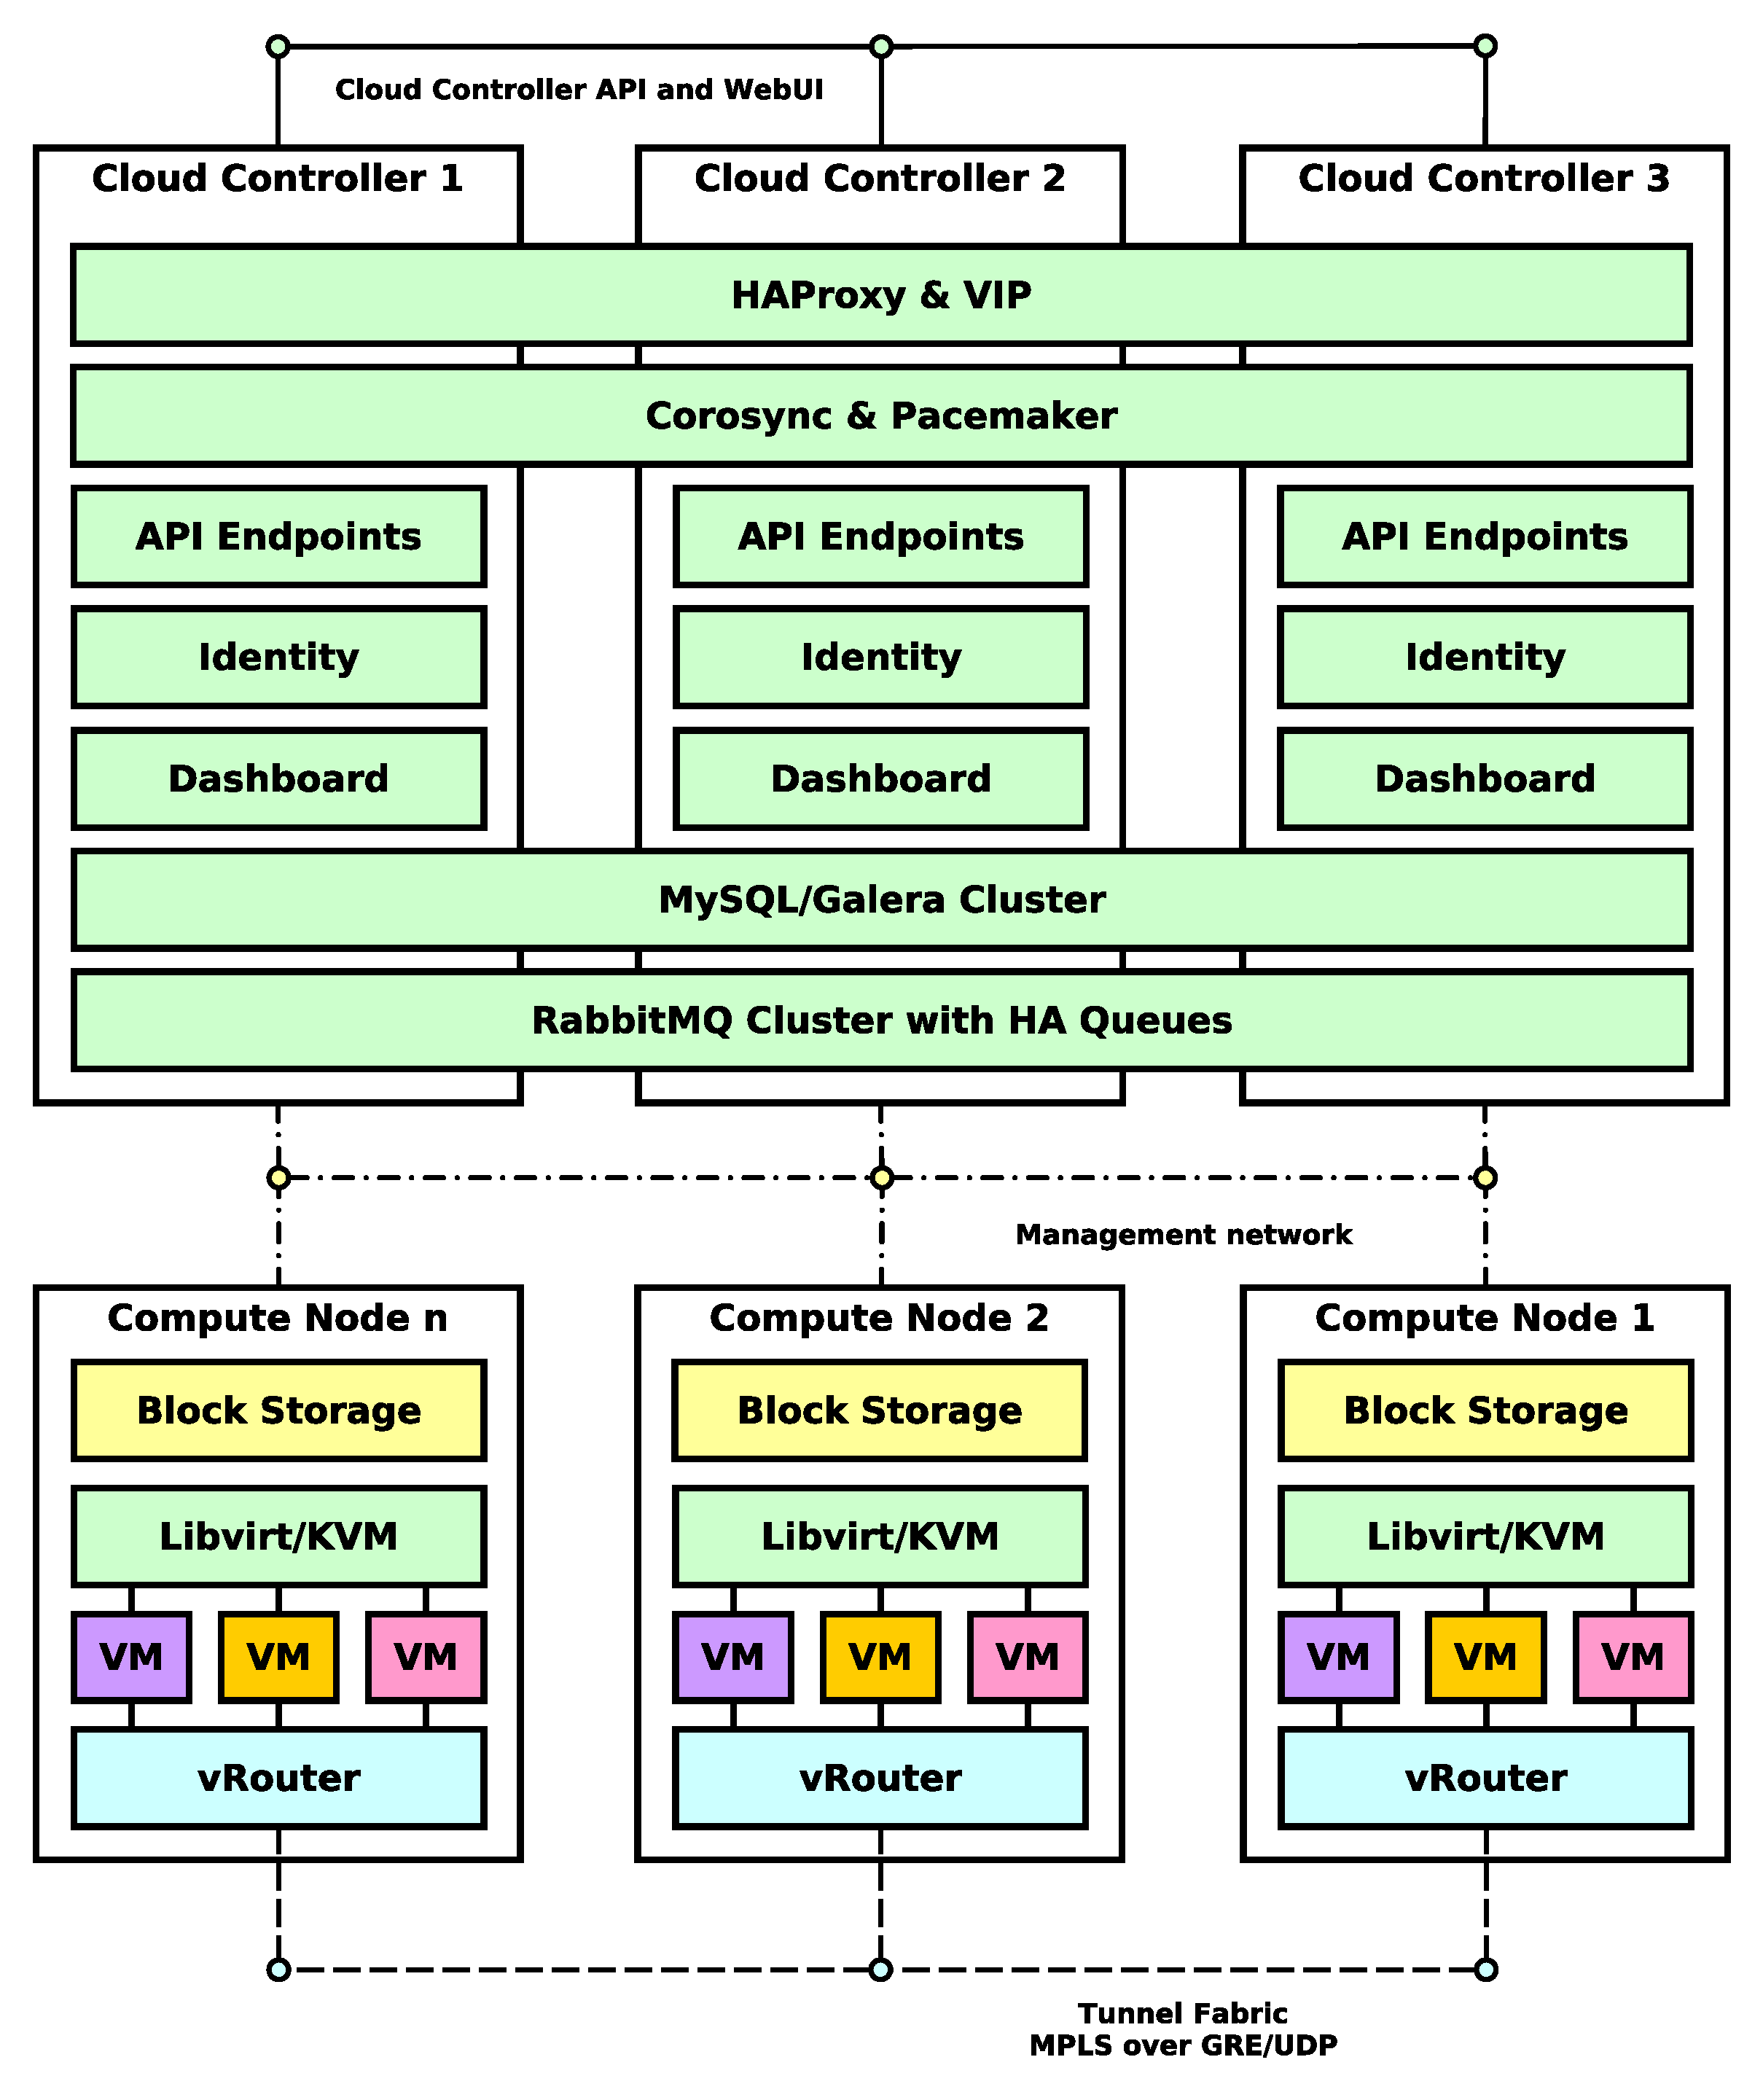
\includegraphics[scale=.2]{img/use_case_ha_gre.eps}
\caption{Locality 1 Architecture}
\label{fig:cm}
\end{figure}

- 20 hypervisors, kvm, ovs-gre, local hdd

\subsubsection{Locality 2}

At Cloudlab in datacenter in Pisek we tested

\begin{figure}[!h]
\centering
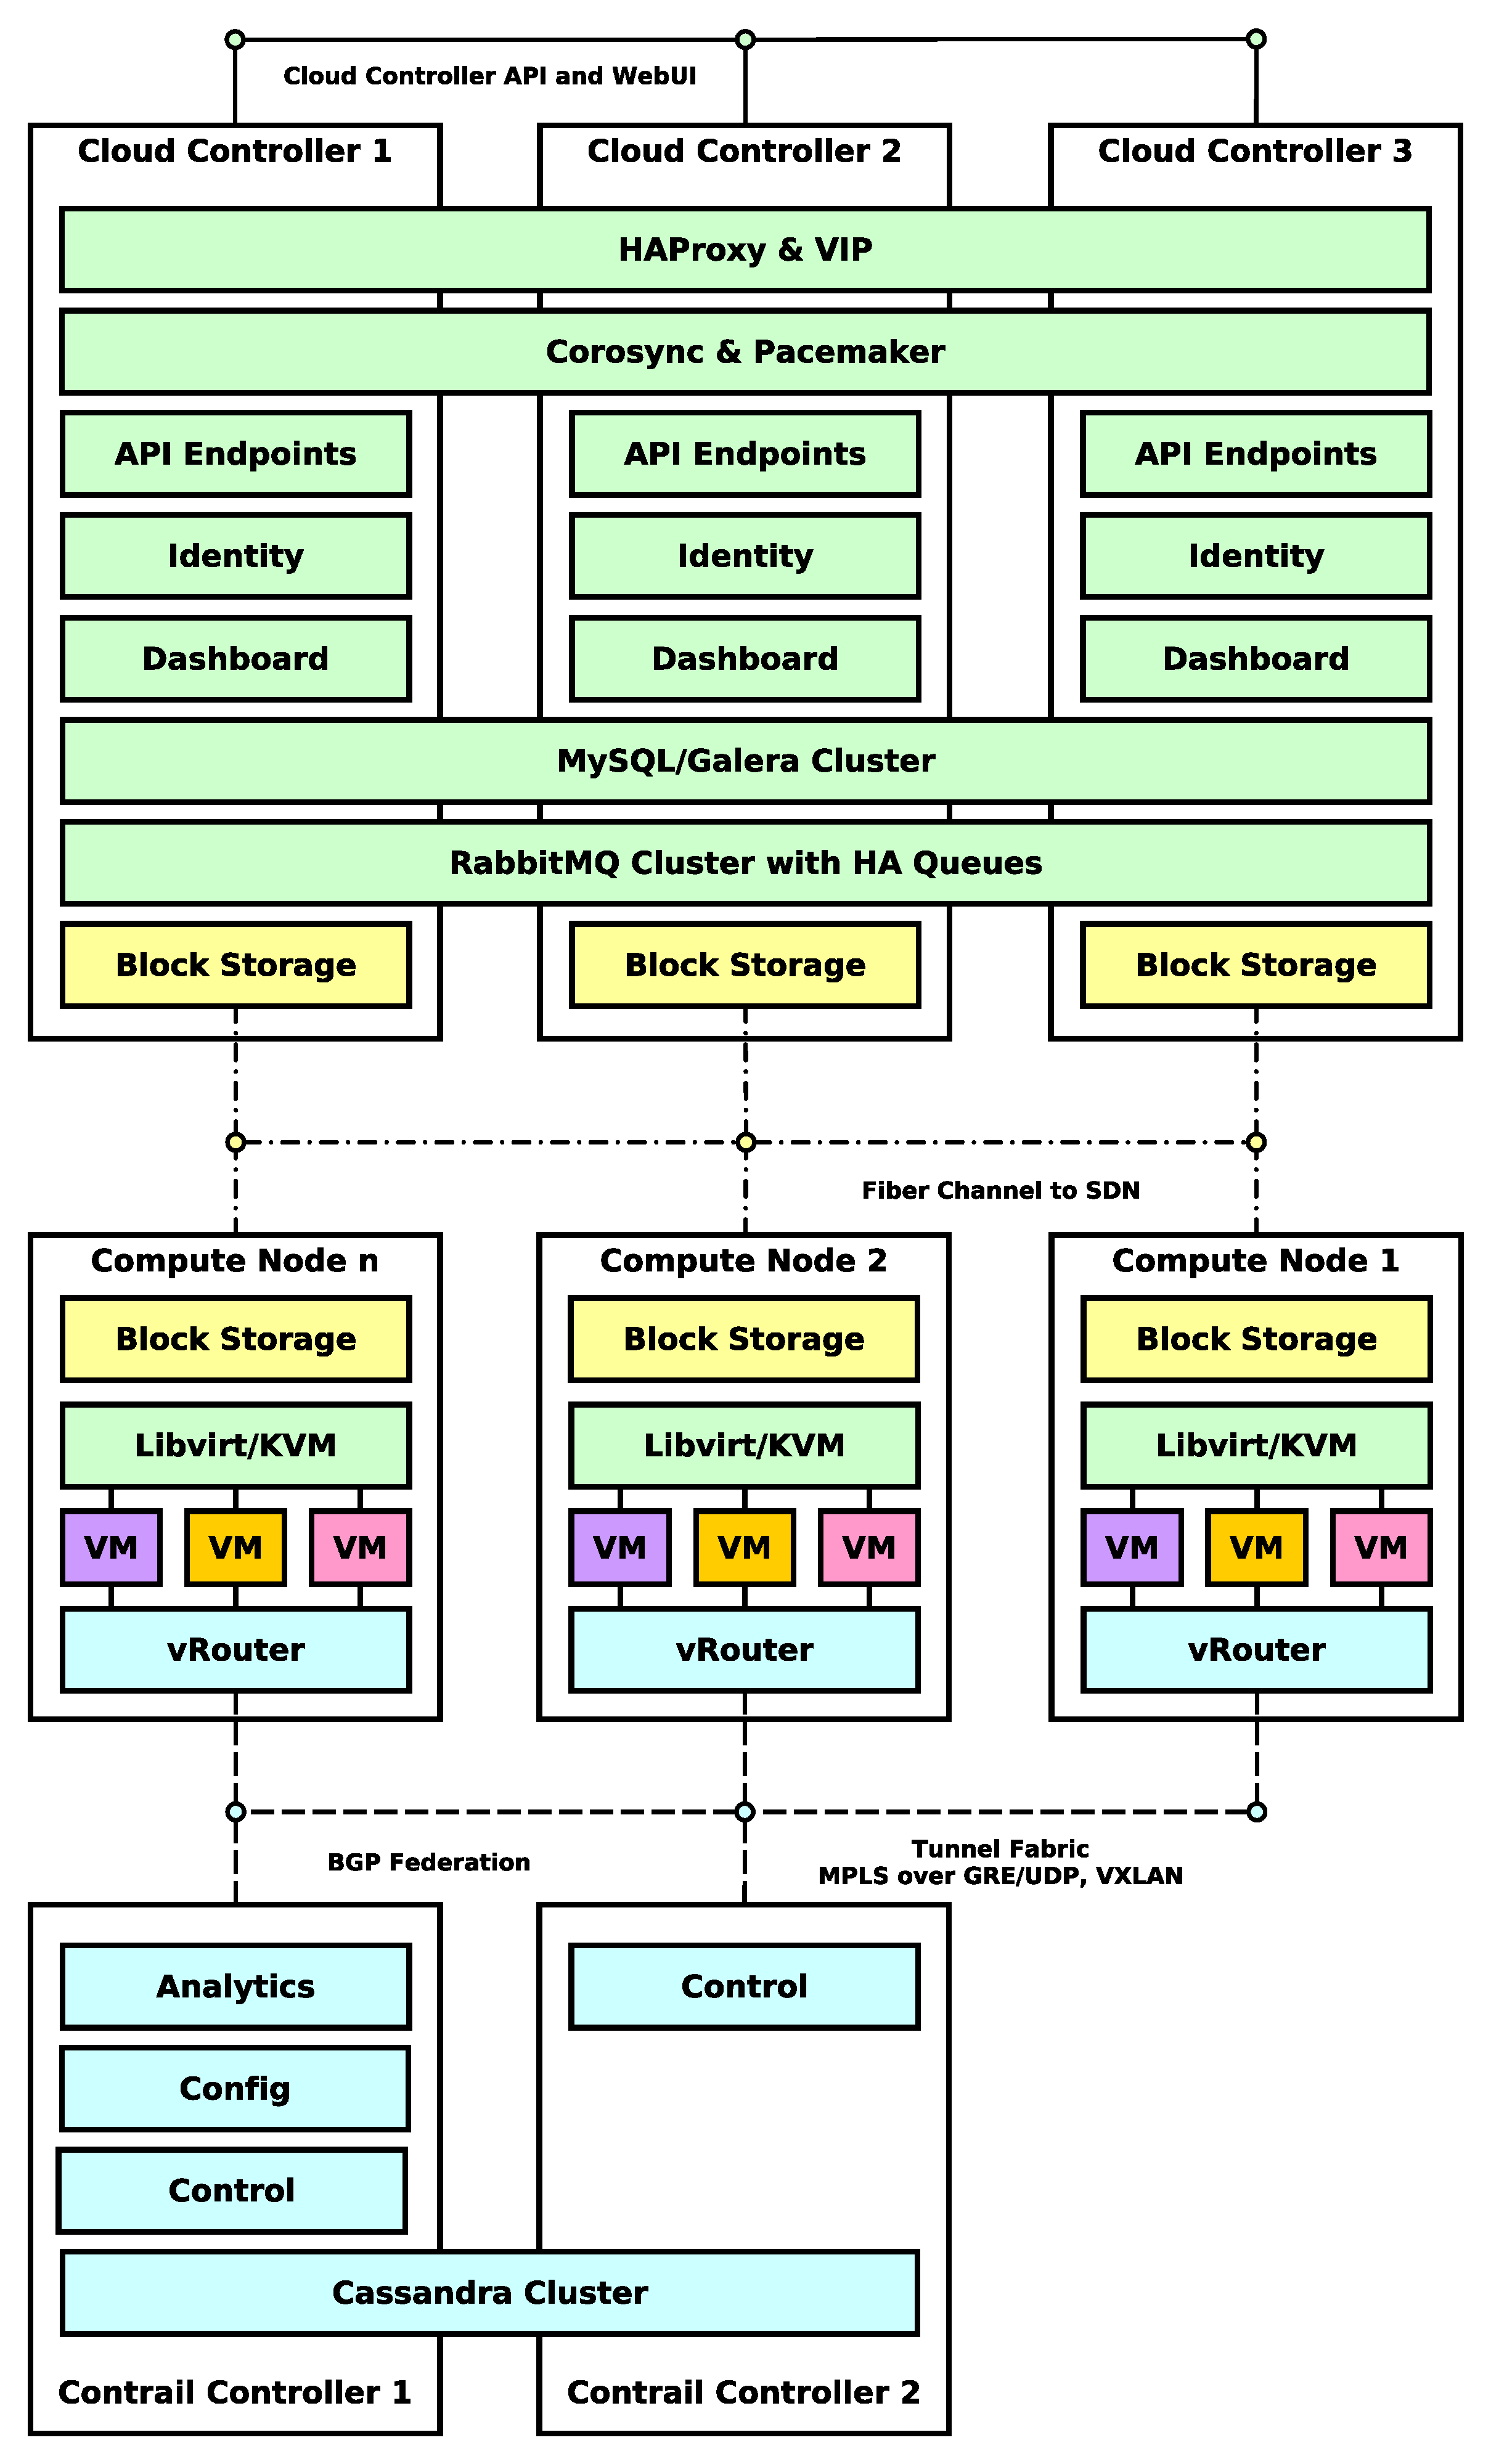
\includegraphics[scale=.2]{img/use_case_ha_sdn.eps}
\caption{Locality 2 Architecture}
\label{fig:cm}
\end{figure}

- 4 hypervisoers, kvm, sdn-contrail, san

\subsubsection{Locality 3}

At Cloudlab in datacenter in Pisek we tested

%\begin{figure}[!h]
%\centering
%\includegraphics[scale=.2]{img/use_case_l2_flat.eps}
%\caption{Locality 3 Architecture}
%\label{fig:cm}
%\end{figure}


- 3 hypervisors, ... l2 networking 

